\begin{figure}[h]
    \centering
    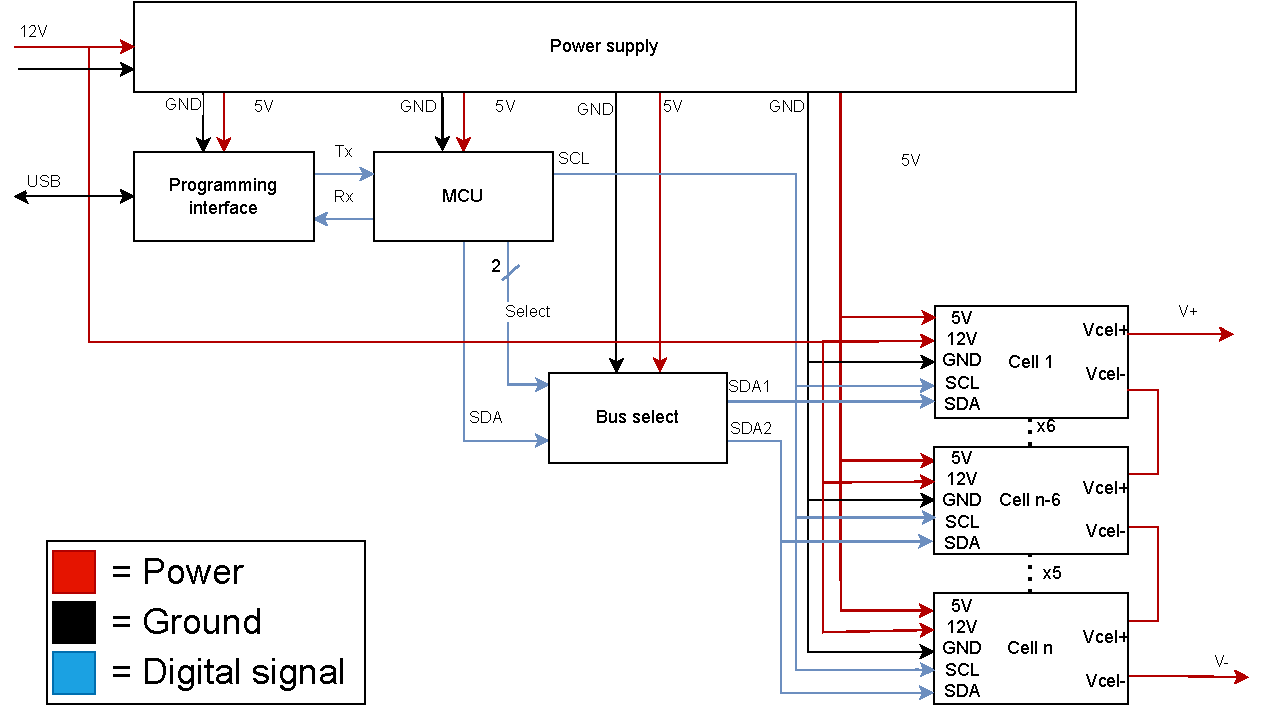
\includegraphics[width=0.5\textwidth]{architecture_2nd_iteration.pdf}
    \caption{Architecture block diagram of the 2nd iteration of the emulator.}
    \label{fig:2nd_architecture}
\end{figure}

The second iteration of the design is made modular, in order to be able to work
 with multiple cells. This is done by implementing a model board
PCB and a cell board PCB. The model board houses 14 slots for cell boards to be 
connected to. This means that as many cells (up to 14) can be used (regardless 
of the slot position). An overview of the architecture is visible in 
Fig. \ref{fig:2nd_architecture}.

    \subsubsection{Model board}
    The model board consists of a 5 V power supply, the microcontroller, a USB 
    conneciton and 14 cell slots. The following is being transmitted at the
    cell slots:

    \begin{itemize}
        \item 12 V from the external power supply
        \item GND
        \item 5 V from the on-board power supply
        \item SDA
        \item SCL
    \end{itemize}

    \subsubsection{Cell board}
    The cell board has an isolated voltage barrier. The incoming 12 V is 
    converted into isolated 9 V using an isolated DC-DC converter, and the data is
    transmitted through the barrier using a bidirectional I2C isolator.

    On the isolated side a voltage regulator provides 
    the 5 V needed to power everything. There is the digital potentiometer
    and the sinking and sourcing circuitry. There are also the address pins, which
    should be soldered in order to provide an address so that every cell board that 
    is connected to the model board can be distinguished.
    The architecture of the single cell can be seen in Fig. 
    \ref{fig:2nd_architecture_cell}.

    \begin{figure}[h]
        \centering
        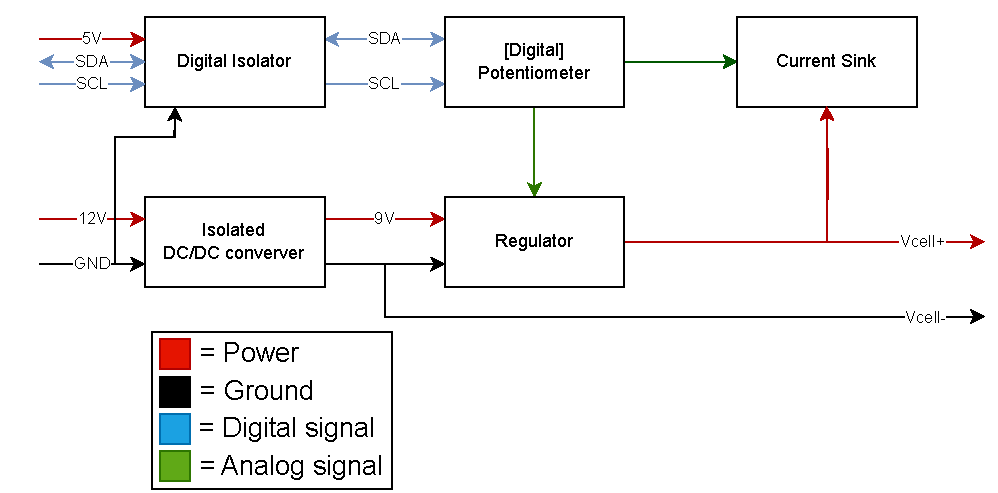
\includegraphics[scale=0.47]{architecture_single_cell.pdf}
        \caption{Architecture block diagram of the cell board.}
        \label{fig:2nd_architecture_cell}
    \end{figure}
